\documentclass[12pt,a4paper,twoside,openany]{book}
\usepackage{textcomp}
\usepackage[T1]{fontenc}
\usepackage[utf8]{inputenc}
\usepackage[italian]{babel}
\usepackage{pdfpages}
\usepackage{graphicx}
\usepackage{rotating}
\usepackage[formats]{listings}
\usepackage{caption}
\usepackage{float}
\usepackage{booktabs}
\usepackage{picture}
\usepackage{multirow}
\usepackage{pifont}
\usepackage[hidelinks]{hyperref}
%codice per mettere logo in sfondo ad ogni pagina
\usepackage{eso-pic}


\AddToShipoutPicture
{
  \put(\LenToUnit{.4\textwidth}, \LenToUnit{.5\textheight}){
\includegraphics{Immagini/logo}}%
}


\makeatletter
\newcommand{\lstuppercase}{\uppercase\expandafter{\expandafter\lst@token\expandafter{\the\lst@token}}}
\newcommand{\lstlowercase}{\lowercase\expandafter{\expandafter\lst@token\expandafter{\the\lst@token}}}
\makeatother

\lstdefinelanguage{myLang}
{
	morekeywords={
		select, from, on, where, group, by, order, sort, join, and, int, string, load, create, into, overwrite, if, table, not, exists, data, inpath, row, format, delimited, fields, terminated, by, stored, as, textfile, FROM, ON, WHERE, GROUP, BY, ORDER, SORT, JOIN, AND, INT, STRING, CREATE, LOAD, DATA, INPATH, OVERWRITE, INTO, TABLE, IF, NOT, EXISTS
	}
}

\lstset{
	language=myLang,
	basicstyle=\ttfamily,
	keywordstyle=\lstuppercase\color{blue}\bfseries,commentstyle=\color{green}\bfseries, stringstyle=\color{red},
	showstringspaces=false, frame=single, numbers=left, numbersep=5pt, numberstyle=\tiny\color{black}, breaklines=true,flexiblecolumns=true,
	inputpath=Sorgenti/,
	sensitive=false
}

%\lstset{basicstyle=\footnotesize\ttfamily\color{black}, language=C,keepspaces=true, format=C, inputpath=Sorgenti/,tabsize=2, keywordstyle=\color{blue}\bfseries,commentstyle=\color{green}\bfseries, stringstyle=\color{black}, showstringspaces=false, frame=single, numbers=left, numbersep=5pt, numberstyle=\tiny\color{black}, breaklines=true,flexiblecolumns=true}

%NOTA: Per ogni nuovo capitolo inserito: creare una cartella col nome dell'esercizio in Immagini ed inserirvi tutte le immagini relative all'esercizio. In seguito inserire il path nell'istruzione graphicspath secondo la sintassi {Immagini/NomeCartellaImmaginiEsercizio/} senza separazione con virgole. Notare lo slash dopo il nome della cartella per indicare che il nome inserito è una cartella.
\graphicspath{{Immagini/}}
\author{Andrea Scognamiglio - Mtr M63/598 \\ Cristian Tommasino - Mtr. M63/615}
\title{
	\centering
	\textbf{Influence Maximization}
}
\date{}

\pagestyle{plain}

\begin{document}
\frontmatter
\maketitle
\setcounter{page}{1}
\tableofcontents
\mainmatter
% !TEX root = ./main.tex
% !TEX encoding = UTF-8 Unicode
% !TEX program = pdflatex
% !TeX spellcheck = it_IT

\chapter{Introduction} \textit{"Yelp è un social network in cui le persone si
scambiano pareri,  opinioni e “dritte” sui posti migliori del luogo in cui
abitano e di  quelli in cui vanno per lavoro, viaggio o altri motivi."}
\footnote{Claudia Resta - Community di Yelp}\\\\
La mission di questo elaborato è
analizzare un dataset fornito da Yelp,  contenente informazioni riguardanti
differenti business, utenti ed un  loro sottoinsieme di recensioni effettuate,
al fine di individuare gli  utenti più influenti della rete.\\
 In particolare,
quello della \textbf{Influence Maximization} è il  problema di trovare un
piccolo \textit{subset} di nodi in una social  network tale da  massimizzare la
diffusione di influenza  (\textit{spread influence}).

\include{data set_Originale}
% !TEX root = ./main.tex
% !TEX encoding = UTF-8 Unicode
% !TEX program = pdflatex
% !TeX spellcheck = it_IT

\chapter{Scelta Architetturale}
In questo capito sarà mostrata l'architettura del sistema utilizzato per
la risoluzione del problema di \textbf{Influence Maximization}. Il sistema è formato da un
livello di data-storage e un livello di elaborazione.

\section{MongoDB}
Nel livello data-storage del sistema, come da requisiti, si richiede l'utilizzo di un database
\textbf{NoSQL}.\\
Esistono diversi tipi di database NoSQL, tra cui: \textbf{chiave-valore}, \textbf{colonnari},
\textbf{graph-db} e \textbf{documentali}.\\
Nel caso in esame, dopo aver visionato i dati a disposizione, si scelto
un database documentale, in particolare \textit{\textbf{MongoDB}}.\\
I database documentali sono adatti alla memorizzazione di dati aggregati, ma non
adatti all'esecuzione di query complesse.\\
Infatti in tali database ogni record è visto come un documento contente delle
caratteristiche, il cui accesso è possibile
solo tramite chiave.\\
Poiché i dati forniti da \textit{Yelp} sono memorizzati in file .json che presentano
delle strutture dati complesse, come ad esempio il campo \textit{Elite} del file
utenti (contenente un array di anni), ed avendo scelto
di non effettuare processing dei dati al livello database, il db più adatto è
risultato essere appartenente a questa vasta famiglia.\\
MongoDB è stato installato per fini didattici su un singolo nodo, di seguito
saranno riportati i dettagli.

\begin{figure}[!htbp]
	
\includegraphics[width=.7\linewidth,keepaspectratio]{mongo.png}
  \caption{MongoDB}
  \label{}
\end{figure}

\section{Apache Spark}
\textbf{Apache Spark} è un framework open source per il calcolo distribuito.\\
Utilizza il paradigma MapReduce in memory riuscendo a raggiungere prestazioni
anche 100 volte superiori a quelle raggiunte da Hadoop.\\
Tale framework è disponibile nei seguenti linguaggi di programmazione:
\begin{itemize}
	\item \textit{\textbf{Scala}};
	\item \textit{\textbf{Java}};
	\item \textit{\textbf{Python}};
	\item \textit{\textbf{R}}.
\end{itemize}
Per poter utilizzare il framework di Apache Spark si è utilizzata la piattaforma
cloud \textbf{Databricks}, che cela tutte la fase di installazione e configurazione
del framework e rende disponibile direttamente all'utente (in versione community)
un \textit{cluster} composto da \textbf{8 core} e \textbf{6GB RAM}.
\begin{figure}[!htbp]
	
\includegraphics[width=.7\linewidth,keepaspectratio]{spark.png}
  \caption{Apache Spark}
  \label{}
\end{figure}

\subsection{Graphx}
Inoltre, per far fronte ad un'elaborazione di \textit{Influence Maximization},
si è dovuto ricorrere a delle strutture a grafi per la rappresentazioni dei nodi,
delle relazioni e per la realizzazione dell'algoritmo di \textit{Spread}.\\
A tal proposito si è fatto uso di \textbf{Graphx}, \textit{API} fornita da Apache
Spark, per la \textit{graph-parallel computation}.

\section{Archittettura}
In definitiva l'architettura del sistema scelto è così definita:
\begin{itemize}
	\item \textbf{MongoDB}: per lo storage dei dati di origine e per dei risultati;
	\item \textbf{Apache Spark}: per il pre-processing dei dati;
	\item \textbf{Graphx} la creazione del grafo e per l'implementazione dell'algoritmo
	 di \textit{Influence Maximization}.
\end{itemize}

\begin{figure}[!htbp]
	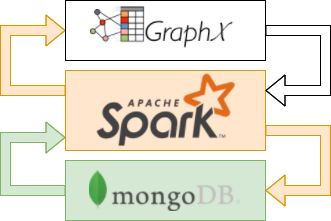
\includegraphics[width=.7\linewidth,keepaspectratio]{architettura.png}
  \caption{Archiettura del sistema}
  \label{sysarch}
\end{figure}

MongoDB è stato installato su un singolo nodo, mentre il framework Apache
Spark con le API annesse di GraphX risiedono nel cloud di Databricks.\\

% !TEX root = ./main.tex
% !TEX encoding = UTF-8 Unicode
% !TEX program = pdflatex
% !TeX spellcheck = it_IT

\chapter{Caricamento dati}
In questo capitolo sono mostrate le operazioni effettuate per il caricamento
dei dati in MongoDB e per il suo collegamento a Databricks.

\section{Caricamento dati in MongoDB}
Come già detto in precedenza, MongoDB è stato installato su di un singolo nodo
e lanciato tramite il comando \textbf{\textit{mongod}}.\\
Su quest'istanza del server è stato possibile importare i dati in formato JSON.\\
Di seguito un esempio di import.

\begin{figure}[!htbp]
	\centering
	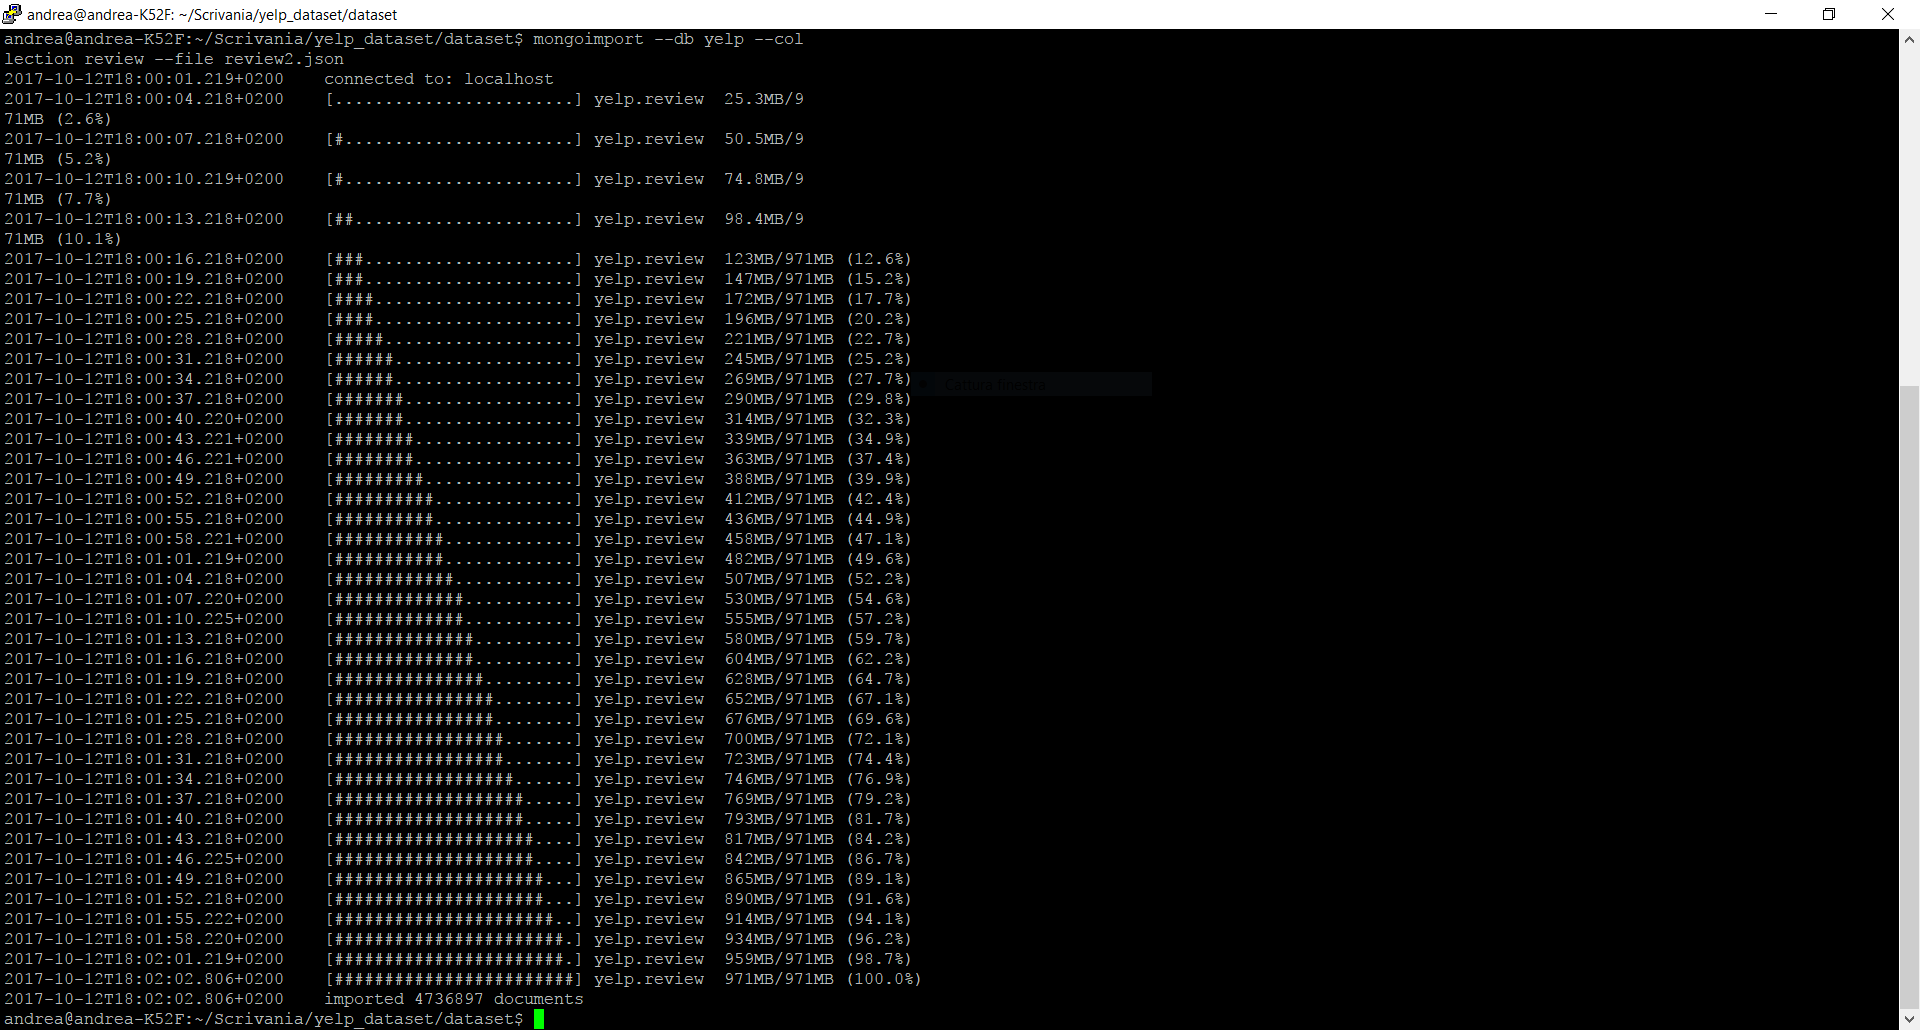
\includegraphics[width=0.9\linewidth,keepaspectratio]{load_on_mongo}
  \caption{Import dati in MongoDB}
  \label{}
\end{figure}
\clearpage

\section{Da MongoDB a Databricks}

Per la connessione di MongoDB a Databricks è stato necessario scaricare il connettore.\\
Quest'ultimo fornisce le API necessarie per il collegamento e l'utilizzo dell'istanza del database.\\
In seguito è riportato il codice per la connessione a MongoDB e l'import dei dati.

\begin{figure}[!htbp]
  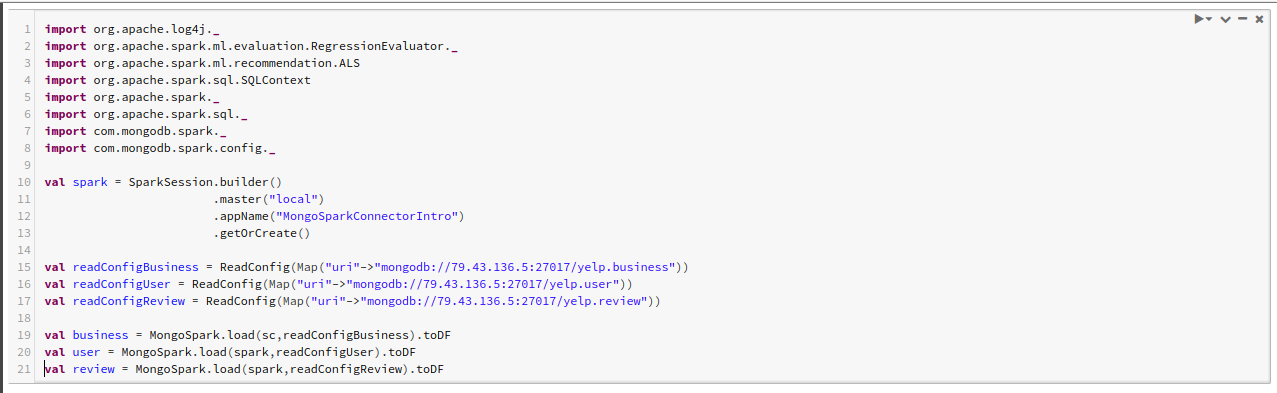
\includegraphics[width=1\linewidth,keepaspectratio]{mongo_spark}
  \caption{Codice per la connessione a MongoDB}
  \label{mongo_spark}
\end{figure}

% !TEX root = ./main.tex
% !TEX encoding = UTF-8 Unicode
% !TEX program = pdflatex
% !TeX spellcheck = it_IT

\chapter{Processing on Databricks}

\section{Drop dati}
In seguito è riportato il codice utilizzato per il drop di informazioni superflue
o ridondanti dai dataframe a disposizione.
\begin{figure}[!htbp]
	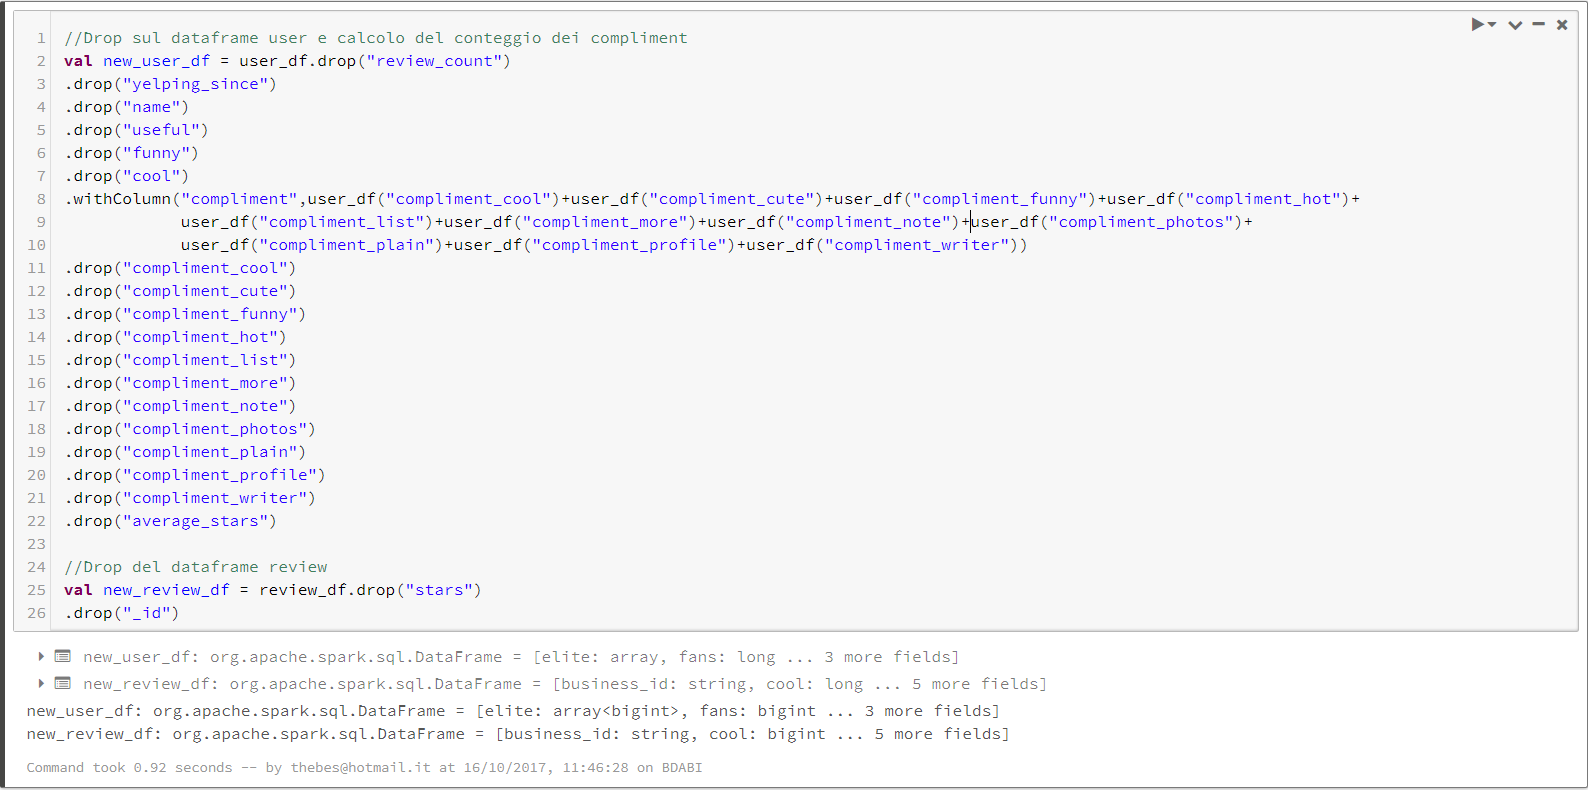
\includegraphics[width=1\linewidth,keepaspectratio]{command_1}
	\caption{Codice per il drop degli attributi superflui}
	\label{command_1}
\end{figure}

\clearpage

\section{Filtraggio Reviews}

\begin{figure}[!htbp]
	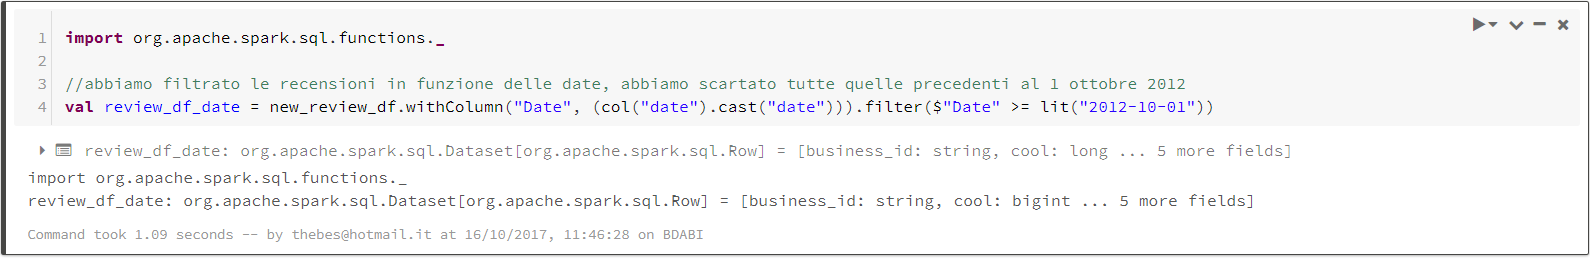
\includegraphics[width=1\linewidth,keepaspectratio]{command_2}
	\caption{Filtraggio delle reviews successive al 1 Ottobre 2012}
	\label{command_2}
\end{figure}

\clearpage

\section{Calcolo attributi di Scoring per Users}
\subsection{Creazione attributo \textit{Elite Score}}
La seguente command filtra gli utenti che hanno il titolo di ``\textit{Elite 2017}''
ed inoltre assegna loro un punteggio dato dalla somma degli anni in cui sono
stati eletti elite.
\begin{figure}[!htbp]
	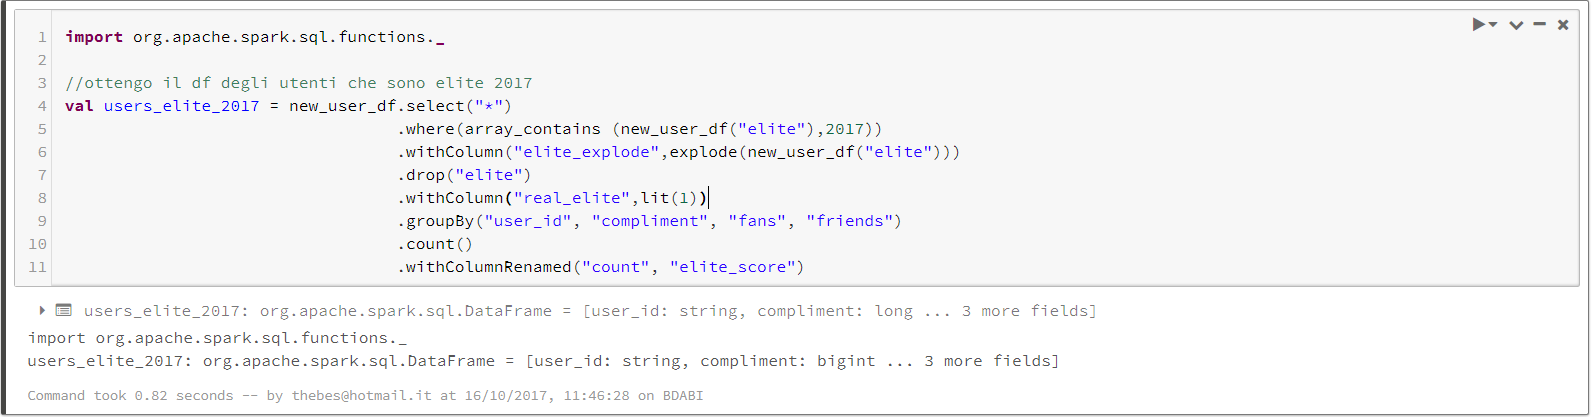
\includegraphics[width=1\linewidth,keepaspectratio]{command_3}
	\caption{Filtraggio degli utenti elite 2017}
	\label{command_3}
\end{figure}

La seguente command filtra gli utenti che non hanno il titolo di ``\textit{Elite 2017}''
ed inoltre assegna loro un punteggio nullo.
\begin{figure}[!htbp]
	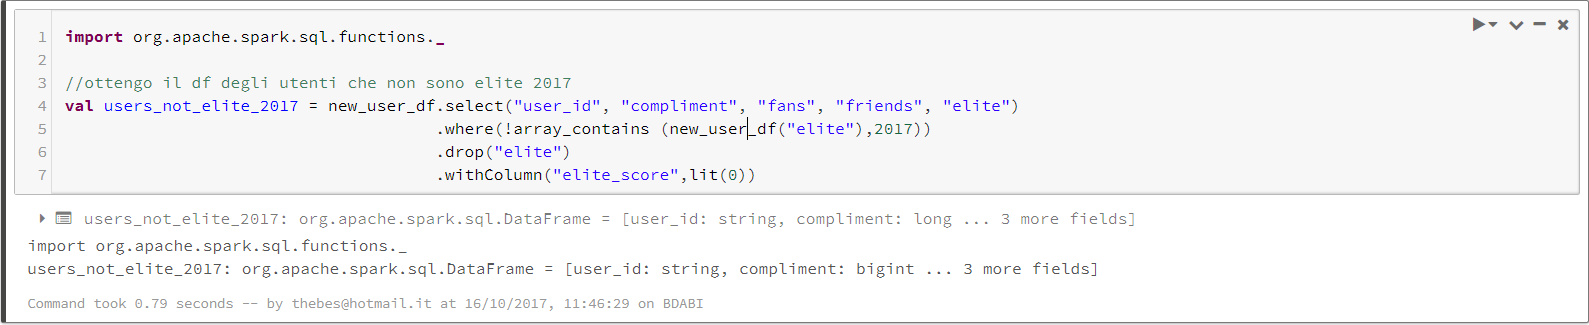
\includegraphics[width=1\linewidth,keepaspectratio]{command_4}
	\caption{Filtraggio degli utenti non elite 2017}
	\label{command_4}
\end{figure}

La seguente command crea un nuovo dataframe Users, aggiungendo il nuovo campo
numerico \textit{elite}
\begin{figure}[!htbp]
	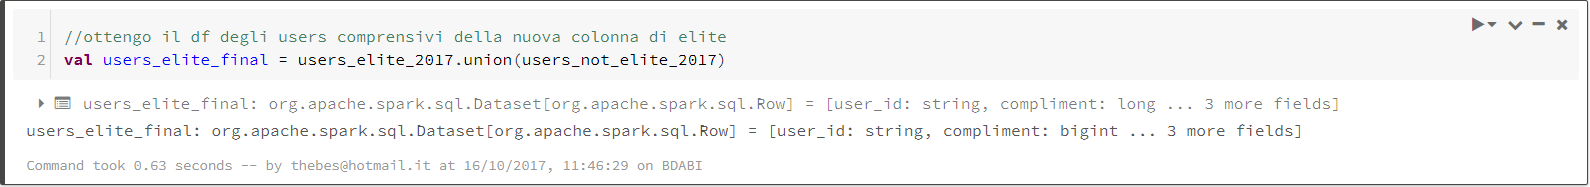
\includegraphics[width=1\linewidth,keepaspectratio]{command_5}
	\caption{Creazione dataframe users contenente il nuovo campo \textit{elite}}
	\label{command_5}
\end{figure}

\subsection{Creazione attributo \textit{Reviews Score}}
La seguente command calcola la combinazione lineare pesata degli attributi \textit{funny},
\textit{cool}, e \textit{useful}.\\
I pesi sono stati assegnati al fine di dar maggiore importanza a quelli che
sono apparsi essere più significativi per l'analisi effetuata.
\begin{figure}[!htbp]
	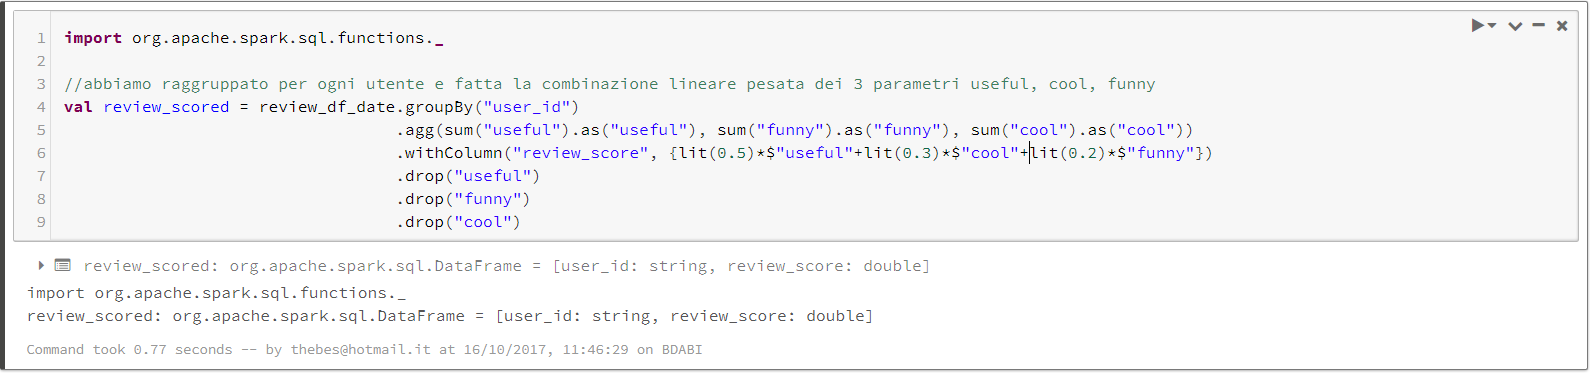
\includegraphics[width=1\linewidth,keepaspectratio]{command_6}
	\caption{Creazione attributo \textit{review\_score}}
	\label{command_6}
\end{figure}

La seguente command crea un nuovo dataframe che comprende il valore review\_score
calcolato.
\begin{figure}[!htbp]
	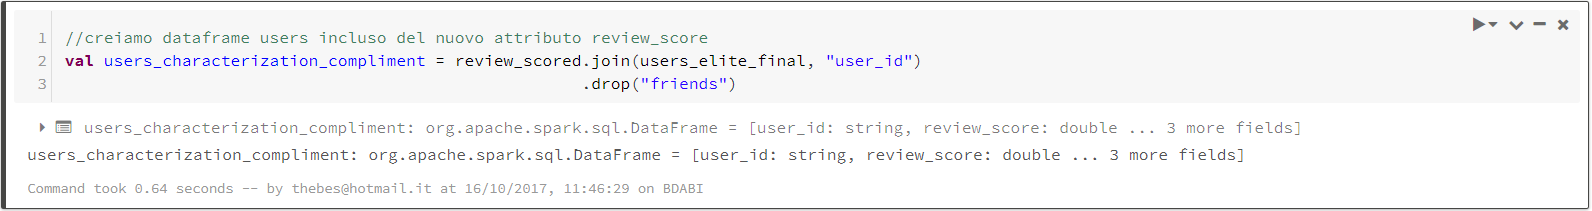
\includegraphics[width=1\linewidth,keepaspectratio]{command_7}
	\caption{Aggiunta \textit{review\_score} al dataframe users}
	\label{command_7}
\end{figure}

\clearpage

\section{Creazione dataframe relazioni user-user con peso archi}
La seguente command prepara un dataframe iniziale user\_relations in cui ogni tupla
soddisfa la proprietà che \textbf{User2} ha recensito almeno \textit{dieci}
business già precedentemente recensiti da \textbf{User1}.
\begin{figure}[!htbp]
	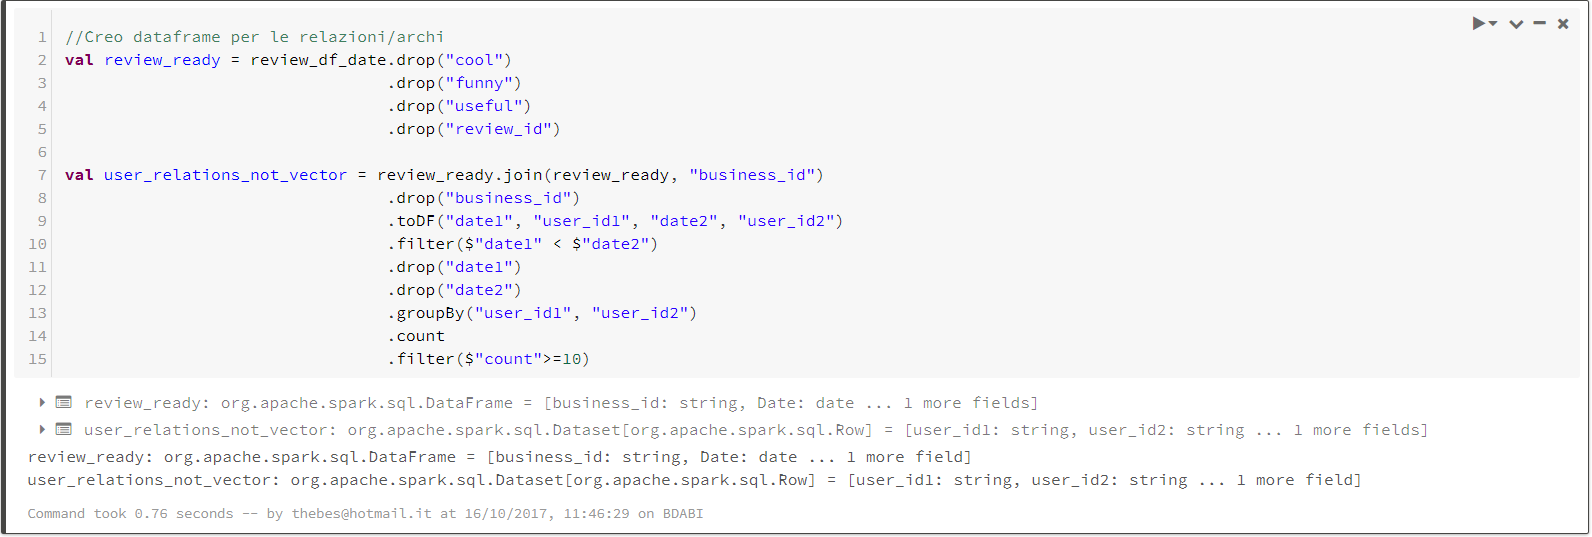
\includegraphics[width=1\linewidth,keepaspectratio]{command_8}
	\caption{Creazione dataframe user\_relations\_not\_vector}
	\label{command_8}
\end{figure}

\clearpage

La seguente command prepara i dati al fine di essere elaborati dallo
\textbf{ScalerModel}, fornito dalle librerie di machine learning di Apache Spark.\\
Questo modello permette di applicare la trasformazione \textit{Z-Score} ai dati,
al fine di normalizzarli.\\
Al termine delle operazioni della command, si ha come dataframe risultante quello
contenente \textbf{UserId1, UserId2, weight\_zscore}, ovvero le relazioni
che caratterizzeranno il grafo della Social Network.

\begin{figure}[!htbp]
	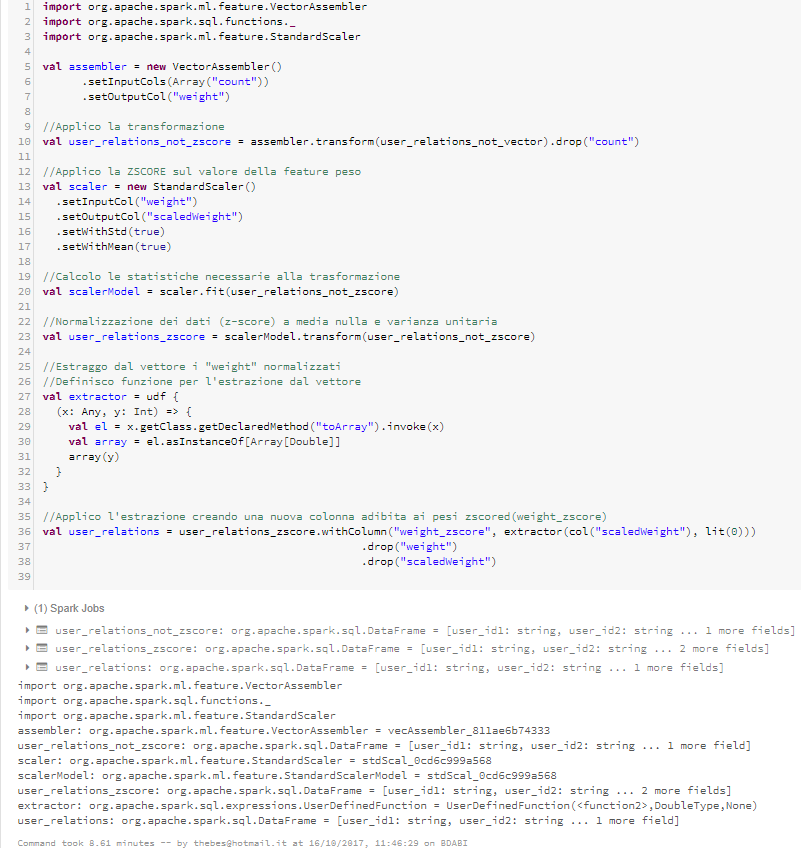
\includegraphics[width=1\linewidth,keepaspectratio]{command_9}
	\caption{Creazione dataframe user\_relations finale}
	\label{command_9}
\end{figure}

\clearpage

\section{Creazione dataframe dei vertici(users) per il grafo}
La seguente command crea un dataframe che, a partire da quello delle relazioni,
prende tutti gli users distinti, così da ottenere i vertici
del grafo.
\begin{figure}[!htbp]
	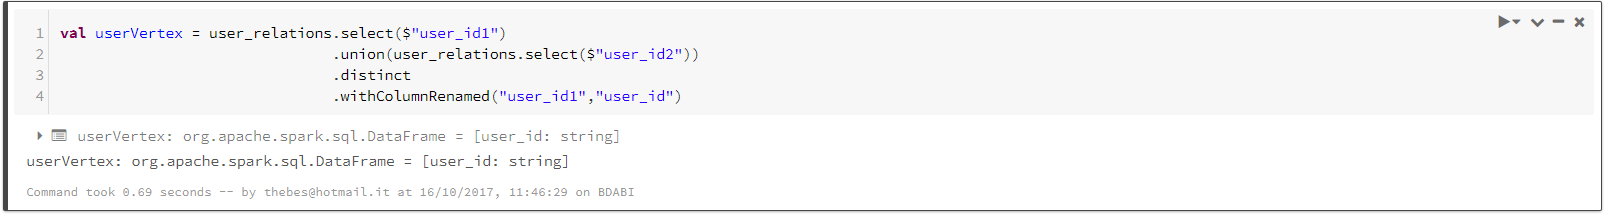
\includegraphics[width=1\linewidth,keepaspectratio]{command_10}
	\caption{Creazione dataframe user\_vertex}
	\label{command_10}
\end{figure}

Le due seguenti command preparano il dataframe per l'applicazione del modello
\textbf{ScalerModel}, al fine di normalizzare i dati prima di combinarli.\\
In seguito si estraggono le quattro \textit{features normalizzate}(review\_score,
compliment, fans, elite\_score) e se ne calcola una combinazione lineare pesata.
\begin{figure}[!htbp]
	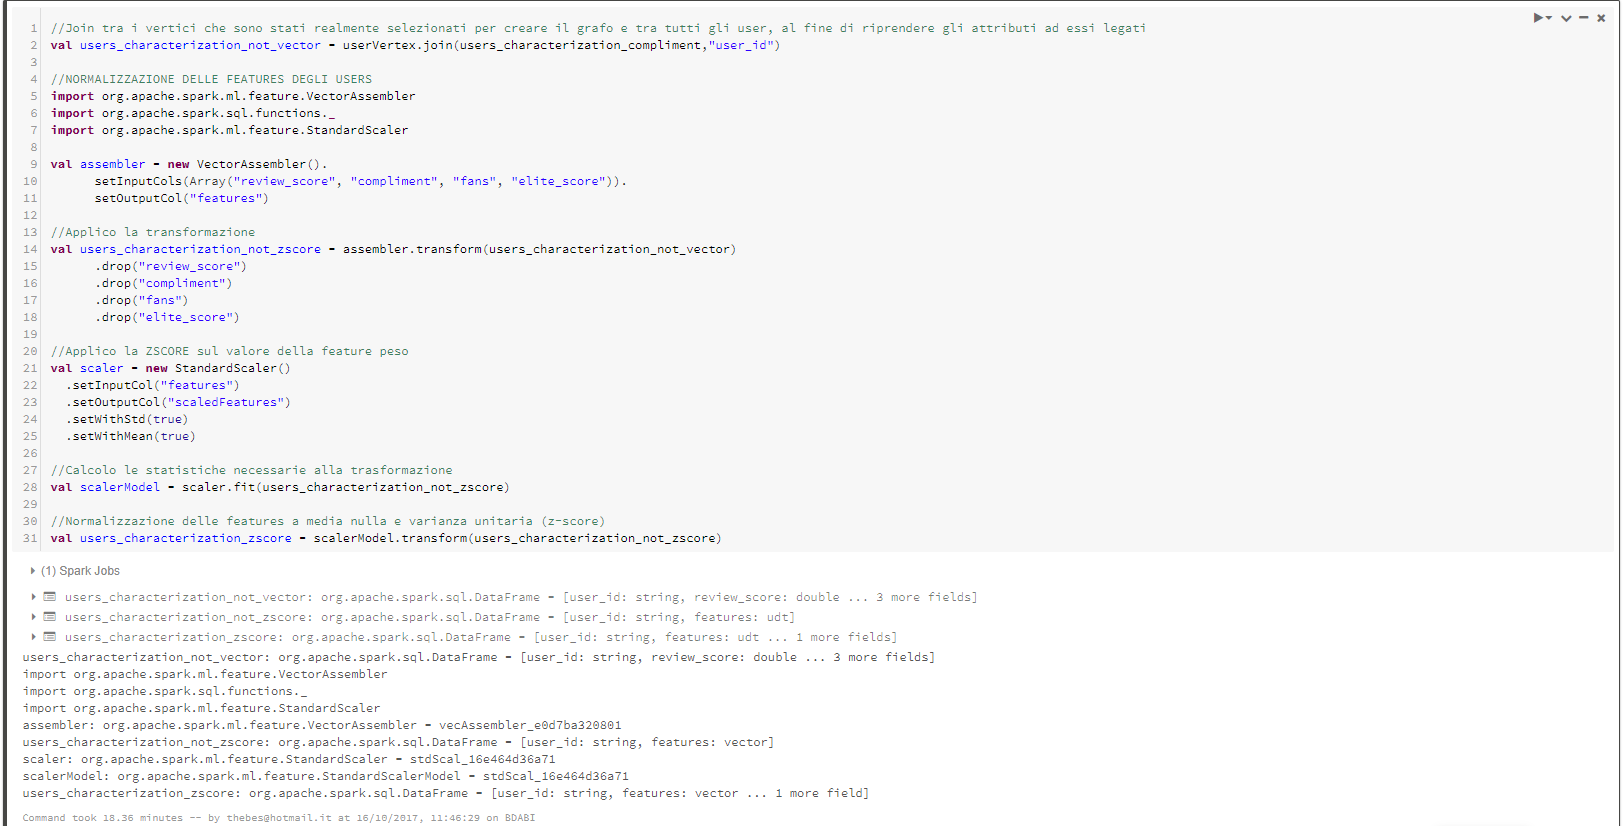
\includegraphics[width=1\linewidth,keepaspectratio]{command_11}
	\caption{Applicazione ScalerModel al dataframe user\_vertex}
	\label{command_11}
\end{figure}

\clearpage

Il risultato finale della seguente command è il dataframe che associa ad ogni user
lo score ad esso calcolato.\\
Questo score è ottenuto come media pesata delle quattro features scelte per
caratterizzare gli utenti.\\
Inizialmente, i pesi sono stati assegnati con egual valore(0.25).\\
Successivamente saranno mostrati differenti esperimenti al loro variare, al fine
di ottenere una copertura maggiore del grafo.
\begin{figure}[!htbp]
 	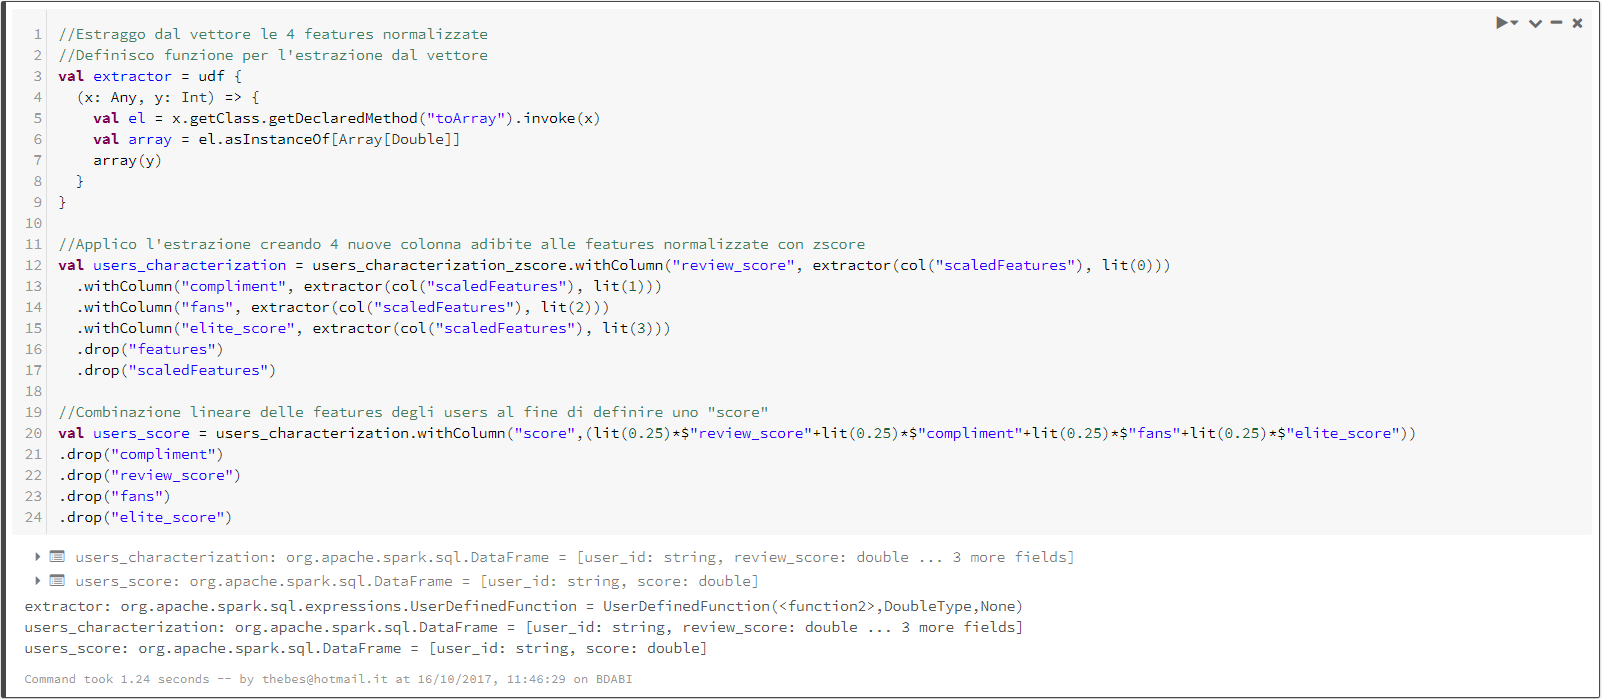
\includegraphics[width=1\linewidth,keepaspectratio]{command_12}
 	\caption{Creazione dataframe contenente user e score calcolato}
 	\label{command_12}
\end{figure}

% !TEX root = ./main.tex
% !TEX encoding = UTF-8 Unicode
% !TEX program = pdflatex
% !TeX spellcheck = it_IT

\chapter{Influence Maximization}
In questo capitolo verrà mostrata la creazione del grafo relativo alla \textit{Social Network}
e l'algoritmo di \textit{Influence Maximization} applicato su di esso.

\section{Creazione del grafo}
Nel precedente capitolo è stata illustrata la caratterizzazione dei nodi (lo score
assegnato ad ogni utente) e la creazione delle relazioni tra essi, con il relativo
peso associato.\\
Per la creazione del grafo è stato utilizzato il framework \textit{\textbf{Graphx}},
il quale permette di definire un oggetto di tipo grafo a partire da un \textit{VertexRDD},
contenente i nodi, e un \textit{EdgeRDD} contenente le relazioni con i relativi pesi.\\
Di seguito è riportato il codice.

\begin{figure}[!htbp]
	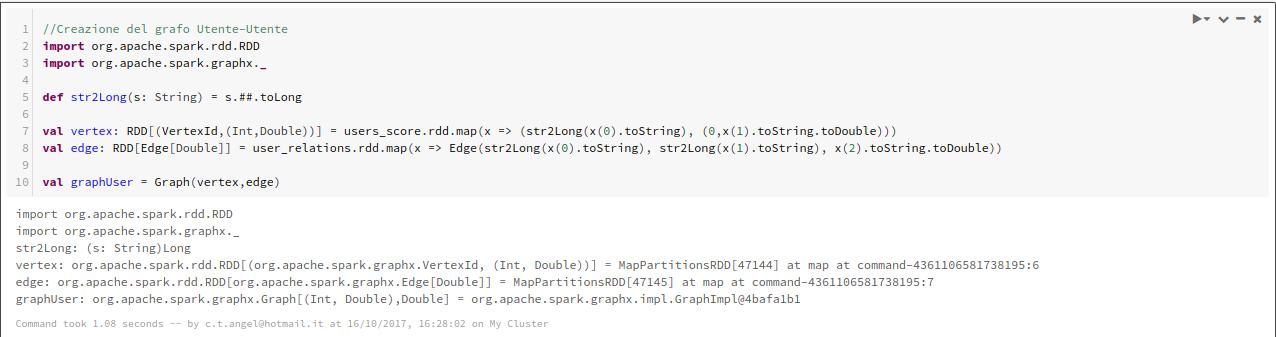
\includegraphics[width=1\linewidth,keepaspectratio]{command_17}
	\caption{Creazione del grafo}
	\label{command_17}
\end{figure}
\clearpage

\section{Algoritmo di Influence Maximization}
L'idea di base dell'algoritmo di Influence Maximization è la seguente: dato il
grafo delle rete sociale ottenuto, avente uno score per ogni nodo ed un peso per
ogni arco, individuare un numero finito di nodi da cui iniziare la copertura del
grafo e propagare l'influence, se e solo se, tale valore supera una soglia prefissata.\\
Per mostrare l'algoritmo utilizzato si consideri il grafo d'esempio in figura.

\begin{figure}[!htbp]
  \begin{center}
    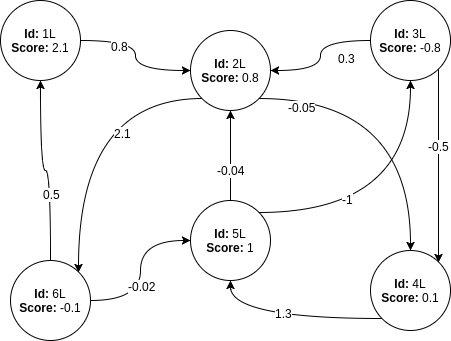
\includegraphics[width=0.6\linewidth,keepaspectratio]{step0}
  	\caption{Grafo d'esempio}
  	\label{step0}
  \end{center}
\end{figure}

\clearpage

Adesso, a fini illustrativi, si considera come nodo di partenza quello avente
score maggiore(evidenziato in verde).\\
Successivamente, invece, verrà illustrata la tecnica utilizzata nell'algortimo di \textit{spread}
per selezionare i nodi di partenza.\\
Nelle figure a seguire, tutti i nodi influenzati saranno evidenziati in verde.
\begin{figure}[!htbp]
  \begin{center}
    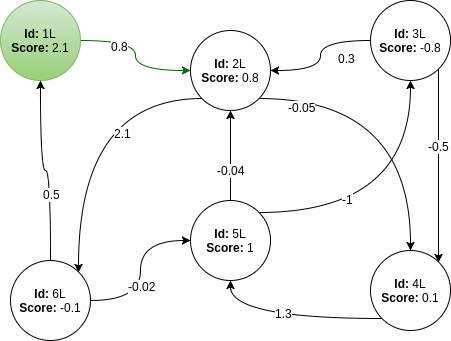
\includegraphics[width=0.6\linewidth,keepaspectratio]{step1}
  	\caption{Scelta nodo di partenza}
  	\label{step1}
  \end{center}
\end{figure}
\clearpage
Ciò che adesso viene illustrato è il meccanismo di diffusione dell'influenza nel
grafo.\\
Il nodo di partenza ha un solo arco in uscita, quindi invierà un messaggio contenente il proprio valore e
la media tra il proprio score ed il peso associato all'arco.\\
Il messaggio ha la seguente struttura $(score\_src, 0.5*score\_src+0.5*weight\_edge)$.\\
Una volta ricevuto il messaggio, il nodo destinazione controlla se il secondo valore è maggiore di una certa soglia,
ad esempio 0.\\
Qualora il confronto risulti positivo, il nodo viene marcato come influenzato ed il
suo score sarà aggiornato con il minimo tra lo score sorgente(moltiplicato per un costante 0.5) ed il proprio score.\\
In \figurename~\ref{step2} è riportato il primo step.\\In particolare si noti che il nodo
risulta essere influenzato, ma il suo score non varia essendo il minimo tra 2.1*0.5 e 0.8.

\begin{figure}[!htbp]
  \begin{center}
    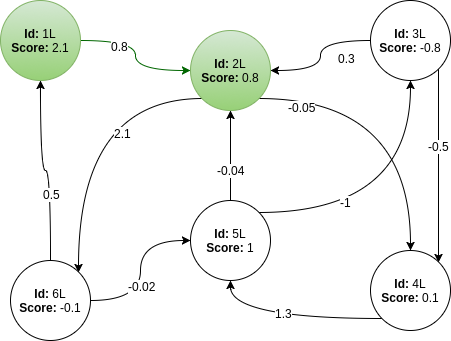
\includegraphics[width=0.6\linewidth,keepaspectratio]{step2}
  	\caption{Passo uno}
  	\label{step2}
  \end{center}
\end{figure}
\clearpage
L'algoritmo continua fintantoché tutti i nodi sono influenzati oppure non esistono più cammini percorribili.\\
Quindi tornando all'esempio, nel secondo step saranno influenzati i nodi \textbf{6L} e \textbf{4L}.

\begin{figure}[!htbp]
  \begin{center}
    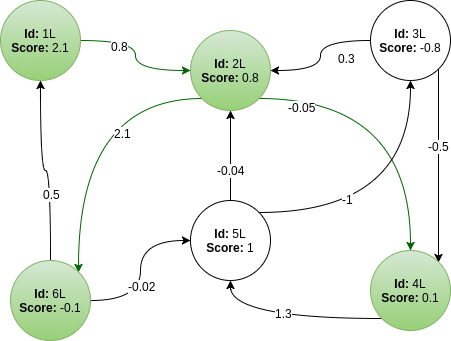
\includegraphics[width=0.6\linewidth,keepaspectratio]{step3}
  	\caption{Passo due}
  	\label{step3}
  \end{center}
\end{figure}
\clearpage
Nel terzo step, si noti che il nodo \textbf{5L} ha due archi in ingesso, sui quali riceve simultaneamente
due messaggi.\\
In tal caso è considerato valido il messaggio avente il secondo campo maggiore.\\
Lo score del nodo 5L è aggiornato, essendo maggiore del valore ricevuto nel messaggio.\\
\begin{figure}[!htbp]
  \begin{center}
    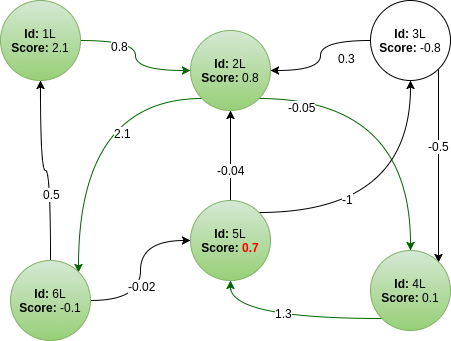
\includegraphics[width=0.6\linewidth,keepaspectratio]{step4}
  	\caption{Passo tre}
  	\label{step4}
  \end{center}
\end{figure}
\clearpage

Nel ultimo step, si noti che il nodo \textbf{3L}, marcato di rosso, non è stato influenzato
in quanto il valore non supera la soglia.
\begin{figure}[!htbp]
  \begin{center}
    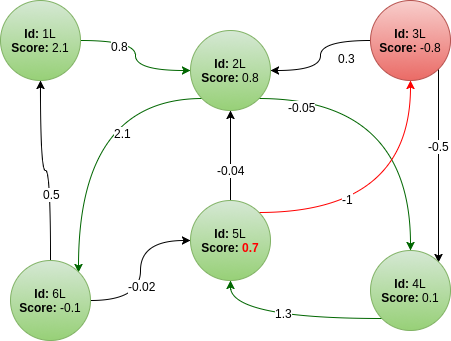
\includegraphics[width=0.6\linewidth,keepaspectratio]{step5}
  	\caption{Passo quattro}
  	\label{step5}
  \end{center}
\end{figure}
\clearpage
\subsection{Scelta degli utenti di partenza}
In questo paragrafo sarà discusso il criterio con cui sono stati scelti gli utenti
di partenza per l'algoritmo di Influence Maximization.\\
In teoria andrebbero testate tutte le possibili combinazioni, in maniera esaustiva,
ma ciò richiederebbe un effort computazionale troppo elevato.\\
L'idea di base è quella di considerare solo un subset di combinazioni, non casuale,
in cui ogni combinazione è costruita con nodi sufficientemente distanti
tra loro, così da assicurare il più possibile una copertura omogenea del grafo.\\
Nel caso in esame, essendo una social network, è possibile utilizzare
come metrica di distanza tra i nodi la loro appartenenza a differenti cluster.\\
Utilizzando un'algoritmo di clustering per grafi, è possibile selezionare
i cluster più fitti e successivamente considerare solo gli N nodi con score maggiore.\\
A causa dei limiti hardware imposti da Databricks, è stato scelto di usare un
massimo di 5 cluster e 2 nodi ciascuno, ottenendo così 32 combinazioni differenti.\\
L'algoritmo di clustering scelto è \textbf{Markov Cluster(MCL)}, basato sulle
catene di Markov.\\
\subsubsection*{Markov Cluster(MCL)}
Per individuare un cluster in un grafo, MCL utilizza una \textbf{matrice stocastica}(matrice
avente elementi non negativi e somma sulle righe o sulle colonne unitaria) ed
il concetto di \textbf{random walks}(cammini casuali tra i nodi).\\
I random walks tra due nodi sono più frequenti se essi appartengono allo stesso gruppo.\\
Studiando la probabilità che un nodo raggiunga un altro nodo del grafo, è possibile
associarlo al cluster corretto.\\
L'algoritmo\footnote{Stijn van Dongen. A stochastic uncoupling process for graphs.
Technical Report INS-R0011, National Research Institute for Mathematics and Computer
Science in the Netherlands, Amsterdam, May 2000.} è diviso in tre fasi, le prime
due simulano i random walks mentre la terza effettua una test di convergenza.\\
Nel dettaglio:
\begin{itemize}
  \item \textbf{Expansion}: calcola il quadrato della Matrice Stocastica;
	\item \textbf{Inflation}: applica il prodotto di Hadamard sulla matrice stocastica
	(prodotto tra due matrici, in cui la risultante ha ad ogni valore \textit{ij} il prodotto
	degli elementi \textit{ij} delle matrici originali e la loro stessa dimensione).
\end{itemize}
Le fasi di Expansion e Inflation sono eseguite in loop più volte finchè un criterio
di \textit{Convergenza} stabilisce che la nuova matrice risultante sia stabile
rispetto l'iterazione precedente.\\
Nel caso non si ottenga la convergenza, esiste un criterio di stop di "sicurezza"
per evitare l'esecuzione dell'algoritmo all'infinito(o per un periodo
inaccettabilmente elevato).\\
Di seguito è riportato il codice in cui è utilizzato tale algoritmo.
\begin{figure}[!htbp]
  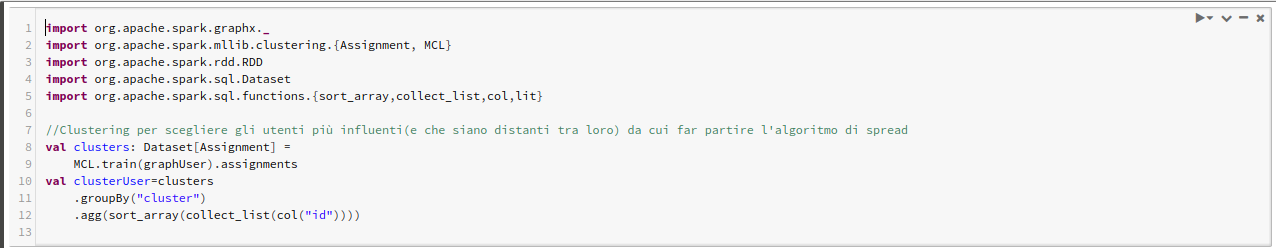
\includegraphics[width=1\linewidth,keepaspectratio]{command_18}
  \caption{Clustering}
  \label{command_18}
\end{figure}

\clearpage
Dato che l'algoritmo di clustering utilizzato non considera i valori presenti nei
nodi, al termine del processo di clustering è necessario recuperarne lo score.\\
Di seguito è riportato il codice per l'estrazione dei nodi di partenza.
\begin{figure}[!htbp]
  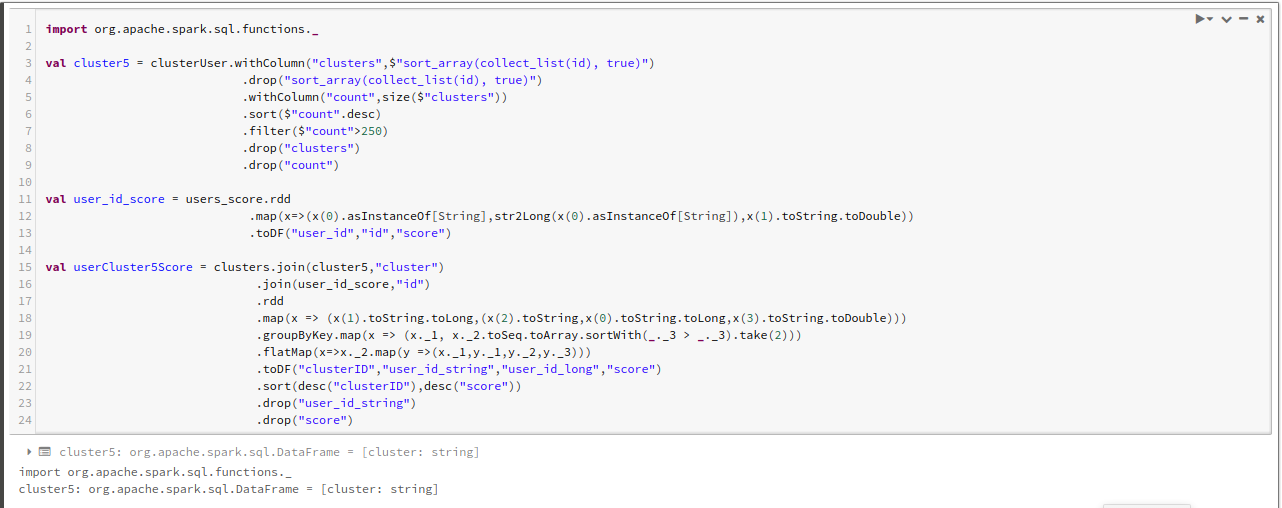
\includegraphics[width=1\linewidth,keepaspectratio]{command_20}
  \caption{Nodi di partenza}
  \label{command_20}
\end{figure}

Nella seguente figura è riportato il codice per la creazione delle combinazioni dei
nodi.
\begin{figure}[!htbp]
  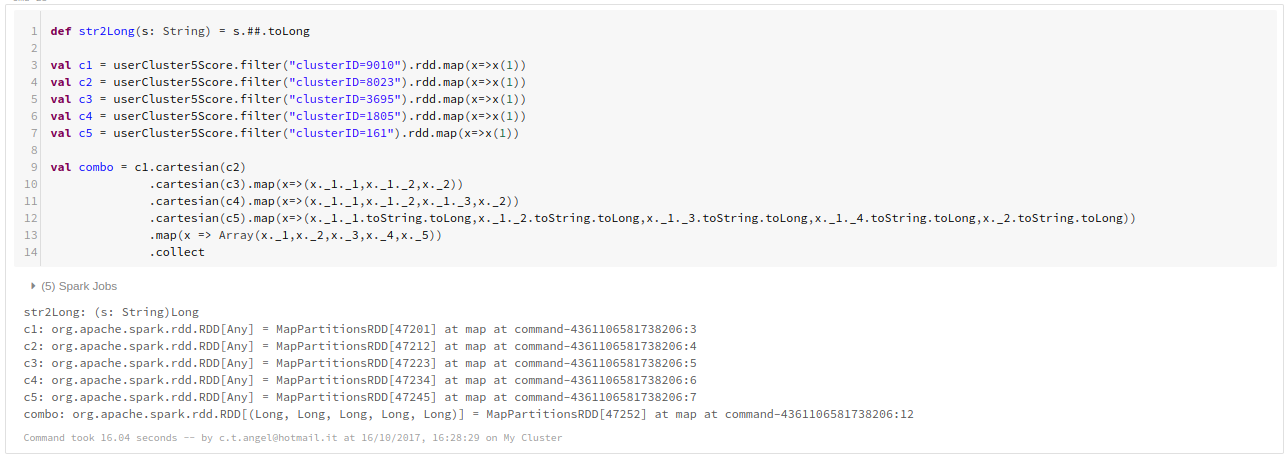
\includegraphics[width=1\linewidth,keepaspectratio]{command_23}
  \caption{Combinazioni dei Nodi}
  \label{command_23}
\end{figure}
\clearpage

\subsection{Scelta della soglia}
Nell'algoritmo di diffusione è stato stabilito di studiare la copertura del grafo
nel caso di due differenti soglie:
\begin{itemize}
	\item Caso A:  media delle \textbf{mediane} degli score degli utenti e dei pesi degli archi;
	\item Caso B:  media delle \textbf{medie} degli score degli utenti e dei pesi degli archi
				(essendo attributi normalizzati con z-score, la media è nulla).
\end{itemize}
In \figurename~\ref{command_24} è mostrato il calcolo della soglia nel caso A.

\begin{figure}[!htbp]
  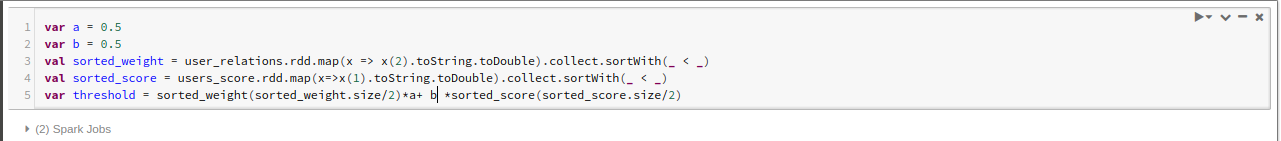
\includegraphics[width=1\linewidth,keepaspectratio]{command_24}
  \caption{Calcolo della soglia}
  \label{command_24}
\end{figure}
\clearpage

\subsection{Implementazione in Scala}
Per l'implementazione dell'algoritmo di \textit{spread}, in Scala, si è fatto uso
della funzione \textit{\textbf{Pregel}}, messa a disposizione dalle API di
\textit{\textbf{Graphx}}.\\
Pregel implementa uno scambio di messaggi tra nodi tramite l'utilizzo di tre
metodi:
\begin{itemize}
	\item \textbf{MergeMsg}: nel caso in cui il nodo riceve messaggi da più sorgenti
	definisce un criterio con cui selezionare solo un messaggio;
	\item \textbf{vProg}: definisce le azioni da compiere nel nodo alla ricezione del messaggio;
	\item \textbf{SendMsg}: definisce i valori da inserire nel nuovo messaggio ed
	il suo criterio di trasmissione.
\end{itemize}
L'esecuzione di \textit{\textbf{Pregel}} è suddivisa in \textbf{Super Step}.\\
In ogni super step, per ogni nodo che riceve un messaggio, sono eseguiti i metodi
sopra descritti.\\
Inoltre possono essere specificati altri parametri come: numero massimo di
iterazioni e messaggio iniziale.\\
Nella figura è riportato il codice per la definizione delle funzioni:
\textbf{MergeMsg}, \textbf{vProg} e \textbf{SendMsg}.
\begin{figure}[!htbp]
  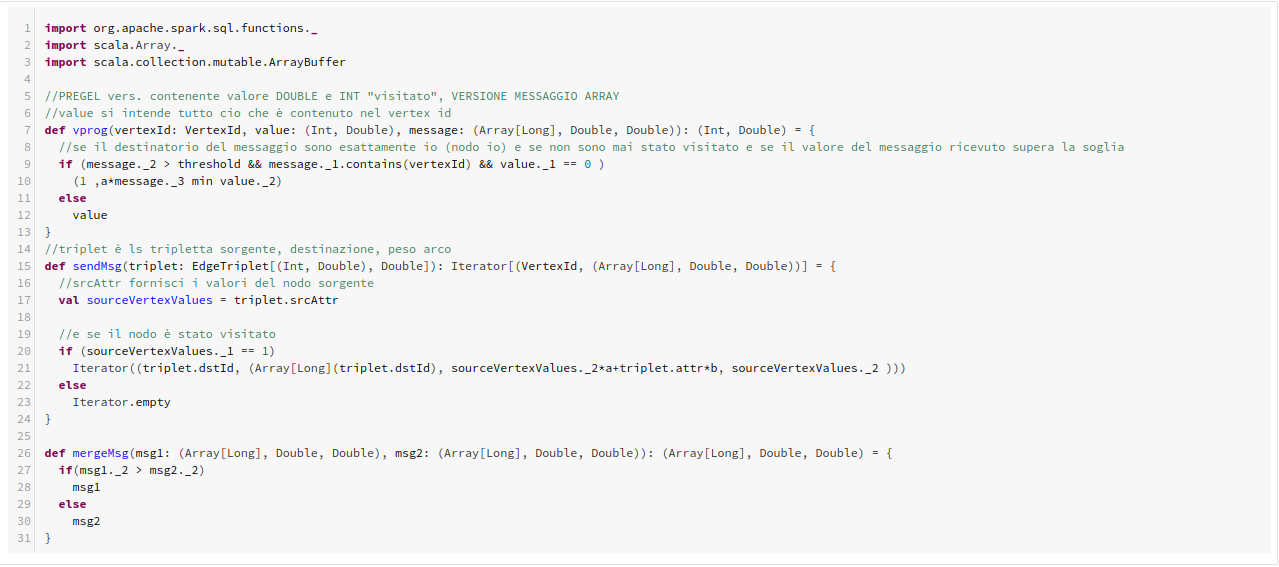
\includegraphics[width=1\linewidth,keepaspectratio]{command_25}
  \caption{Definizione MergeMsg, vProg, SendMsg}
  \label{command_25}
\end{figure}
\clearpage
Scendendo nel dettaglio, in \figurename~\ref{command_25} si osserva che:
\begin{itemize}
	\item in \textbf{MergeMsg} viene scelto, in caso di ricezione simultanea di
	messaggi, quello con valore maggiore;
	\item in \textbf{vProg} viene confrontato il secondo campo del messaggio ricevuto
	con la soglia, se il nodo è un nodo destinazione e se non è ancora
	stato influenzato, nel caso di esito di positivo, la variabile
	\textit{\textbf{influenced}} è settata ad 1 ed il valore del nodo è aggiornato
	con il \textit{min} tra il primo campo del messaggio(moltiplicato per 0.5) ed il suo score;
	\item in \textbf{SendMsg} ogni nodo che è stato influenzato invia un messaggio
	a tutti i suoi vicini.
\end{itemize}
Nel seguente codice è riportato l'algoritmo di \textit{Spread} per ogni
combinazione e l'estrazione del risultato finale avente maggiore copertura.
\begin{figure}[!htbp]
  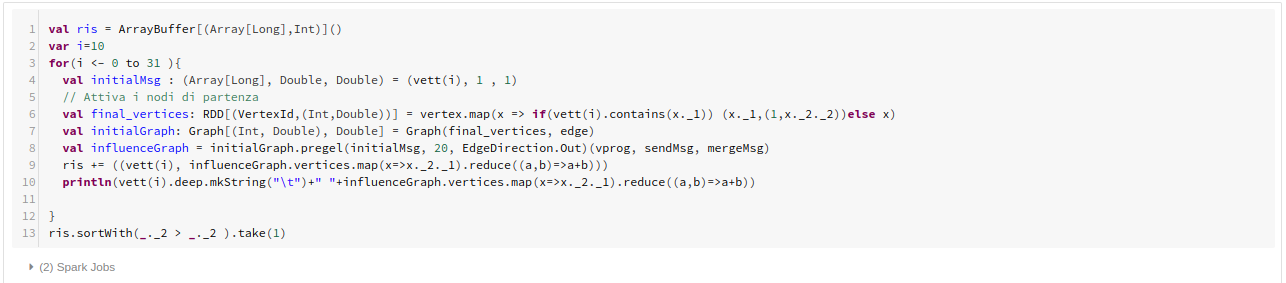
\includegraphics[width=1\linewidth,keepaspectratio]{command_26}
  \caption{Esecuzione Pregel}
  \label{command_26}
\end{figure}
\clearpage

% !TEX root = ./main.tex
% !TEX encoding = UTF-8 Unicode
% !TEX program = pdflatex
% !TeX spellcheck = it_IT

\chapter{Analisi dei risultati}
In questo capitolo saranno mostrati i risultati ottenuti per ogni combinazione
lineare utilizzata.

\section{Scelta dei parametri di Scoring}
Per il tuning dei parametri di scoring si è eseguito l'intero processo più volte
mirando ad ottenere la combinazione che presentasse la copertura del grafo
maggiore.\\
In \figurename~\ref{} è riportata la tabella contente i test effettuati.

\begin{figure}[!htbp]
  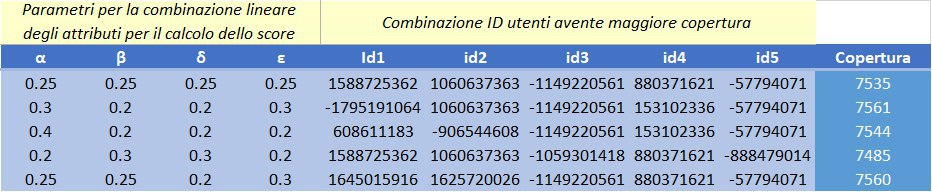
\includegraphics[width=1\linewidth,keepaspectratio]{ris_table}
  \caption{Tabella Risultati}
  \label{ris_table}
\end{figure}

\end{document}
